\documentclass[tikz, border=3.14mm]{standalone}
\usepackage{pgfplots}
\pgfplotsset{compat=1.18}

\begin{document}
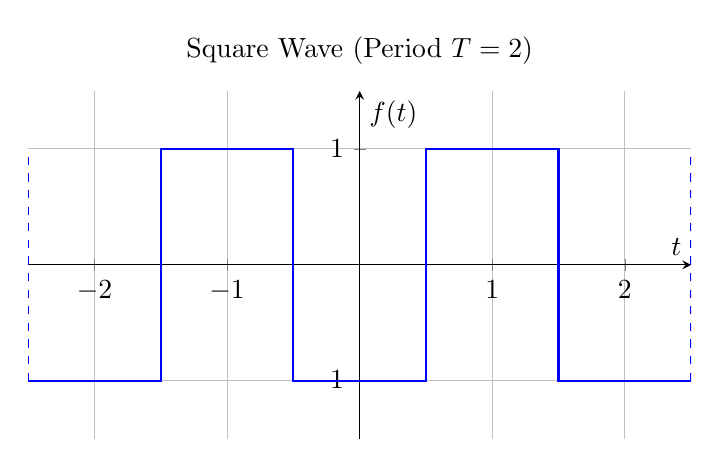
\begin{tikzpicture}
    \begin{axis}[
        axis lines = middle,
        xlabel = {$t$},
        ylabel = {$f(t)$},
        xmin = -2.5, xmax = 2.5,
        ymin = -1.5, ymax = 1.5,
        xtick = {-2, -1, 0, 1, 2},
        ytick = {-1, 1},
        grid = major,
        width = 10cm,
        height = 6cm,
        title = {Square Wave (Period $T=2$)}
    ]
        % Square wave: period 2, cosine-like (even symmetry)
        % High from -0.5 to 0.5, Low from 0.5 to 1.5
        \addplot[
            domain=-2.5:2.5,
            samples=200,
            thick,
            blue,
            const plot
        ] coordinates {
            (-2.5, -1)
            (-2.5, -1)
            (-1.5, 1)
            (-0.5, 1)
            (-0.5, -1)
            (0.5, -1)
            (0.5, 1)
            (1.5, 1)
            (1.5, -1)
            (2.5, -1)
        };
        
        % Vertical lines at jumps
        \draw[blue, thick, dashed] (axis cs:-2.5, -1) -- (axis cs:-2.5, 1);
        \draw[blue, thick] (axis cs:-1.5, -1) -- (axis cs:-1.5, 1);
        \draw[blue, thick] (axis cs:-0.5, -1) -- (axis cs:-0.5, 1);
        \draw[blue, thick] (axis cs:0.5, -1) -- (axis cs:0.5, 1);
        \draw[blue, thick] (axis cs:1.5, -1) -- (axis cs:1.5, 1);
        \draw[blue, thick, dashed] (axis cs:2.5, -1) -- (axis cs:2.5, 1);

    \end{axis}
\end{tikzpicture}
\end{document}
